\chapter{Introduction}
\setcounter{page}{1}
\pagenumbering{arabic}

\shorthandoff{-}

Bacteria exhibit genotypic and phenotypic variability even at the level of genus.
This variability is continuously shaped by natural selection as the cells that are better adapted to the current conditions are more likely to survive and proliferate.
In the case of unicellular organisms, the survival game is more stringent, because they face changing conditions directly, and have limited ability to escape.
Cells must survive for example osmotic stress, nutrient-poor environments, or high UV radiation. They have evolved multiple ways to overcome such conditions, many of which rely on responding to such environmental changes with physiological adaptations.
These are all mediated by sensing external signals and translating them into internal responses.
However, the responses to the same signal might differ among bacteria.
These differences could be driven by other selection forces acting simultaneously or could be a result of previous evolution in response to a similar environment.
In any case, cells which do not manage to adapt to the new conditions are likely to be excluded by natural selection and die.

It is thus essential for a living cell to sense what is happening in the environment and react accordingly and in a timely manner.
If the timescale of an appropriate reaction should be on the order of seconds, there is no time for changes in transcription or translation.
In that case, the cell fate depends on the proteins or other small molecules it has already synthesised.
One example of a fast response to a signal is chemotaxis.
When a motile bacterium occurs in a gradient of an attractant (e.g., nutrients such as sugars or amino acids) or repellent (e.g., toxic metabolites), it swims towards or away from the higher concentration of it, respectively.
The change from a random bacterial walk to active chemotaxis is mediated by a protein CheY.
Its phosphorylation depends on sensing of external signals and determines the probability of flagella rotating clockwise (i.e., cell rotation) switching into counter-clockwise motion (i.e., straight run) \cite{shimizu2010modular, mears2014escherichia}.

On the other hand, if it is advantageous or only necessary to react in minutes or hours, responses can be mediated through translational or transcriptional changes.
Sometimes a quick change in expression can even be detrimental, especially in the case of extensive physiological reprogramming.
Because such alterations consume a lot of energy it might be more profitable for the cell to not respond at once.
Cells might even benefit from not responding at all for some time, for example, if the signal triggering costly response is likely to be transient.
To manage and orchestrate many responses to multiple signals cells evolved a network of extra- and intracellular signalling pathways.

As I focus on transcriptional responses, the following text covers mostly these cases and describes the effects of different mechanisms on the speed of the cell response, transcriptional noise, sensitivity, and epigenetics.
Response times depend on the topology of the circuit, the signals that bacteria have observed previously (memory), and any predictive behaviour that the bacteria are capable of.
By epigenetics or memory, I mean a heritable change in gene expression without simultaneous changes in DNA primary sequence.
The transcriptional noise is understood as variability in gene expression among individual cells with the same genetic background.
Below I go into each of these properties in more detail to establish the current state of the field.
I focus on \tax{E. coli} strains as it is a well-studied model organism, however little is known about its environmental isolates which seems to be adapted to survive and proliferate outside their hosts \cite{byappanahalli2004indigenous, ishii2006presence, somorin2016general}.



\section{Signal recognition}
The first step of cellular response is the sensing of internal and external cues.
There are several means by which bacteria can detect such signals, and these are described below.
However, there is little known about how these different signal sensing mechanisms affect the cell response dynamics and whether they differ in terms of speed, sensitivity, noise or memory.

\subsection{Direct signalling pathways}
Direct signalling occurs when a signal molecule is imported through a cell membrane into the cytosol, or is produced by the cell and subsequently interacts with regulatory proteins.
This is often the case for genes involved in carbohydrate catabolism and amino acid biosynthesis \cite{charlier1992arginine, weickert1992isorepressor, pittard1996various, wheatley2013structural}.
In these cases, the nutrient import into a cell is utilized also for signalling besides consumption purposes.
Physical signals such as UV or heat are also considered direct, although no active import takes place in the signalling.

\subsection{Indirect signalling pathways}
It is not always beneficial for a cell to import signal molecules into the cytosol as some of these might be toxic or simply too big (e.g., host-pathogen cell-cell interactions).
In order to sense environmental cues without the necessity to import them, bacteria possess transmembrane sensory proteins.
Upon binding of a signal molecule by extracellular domain, the protein changes its conformation transferring the received signal into the cell interior.

\begin{figure}[ht!]
  \centering
  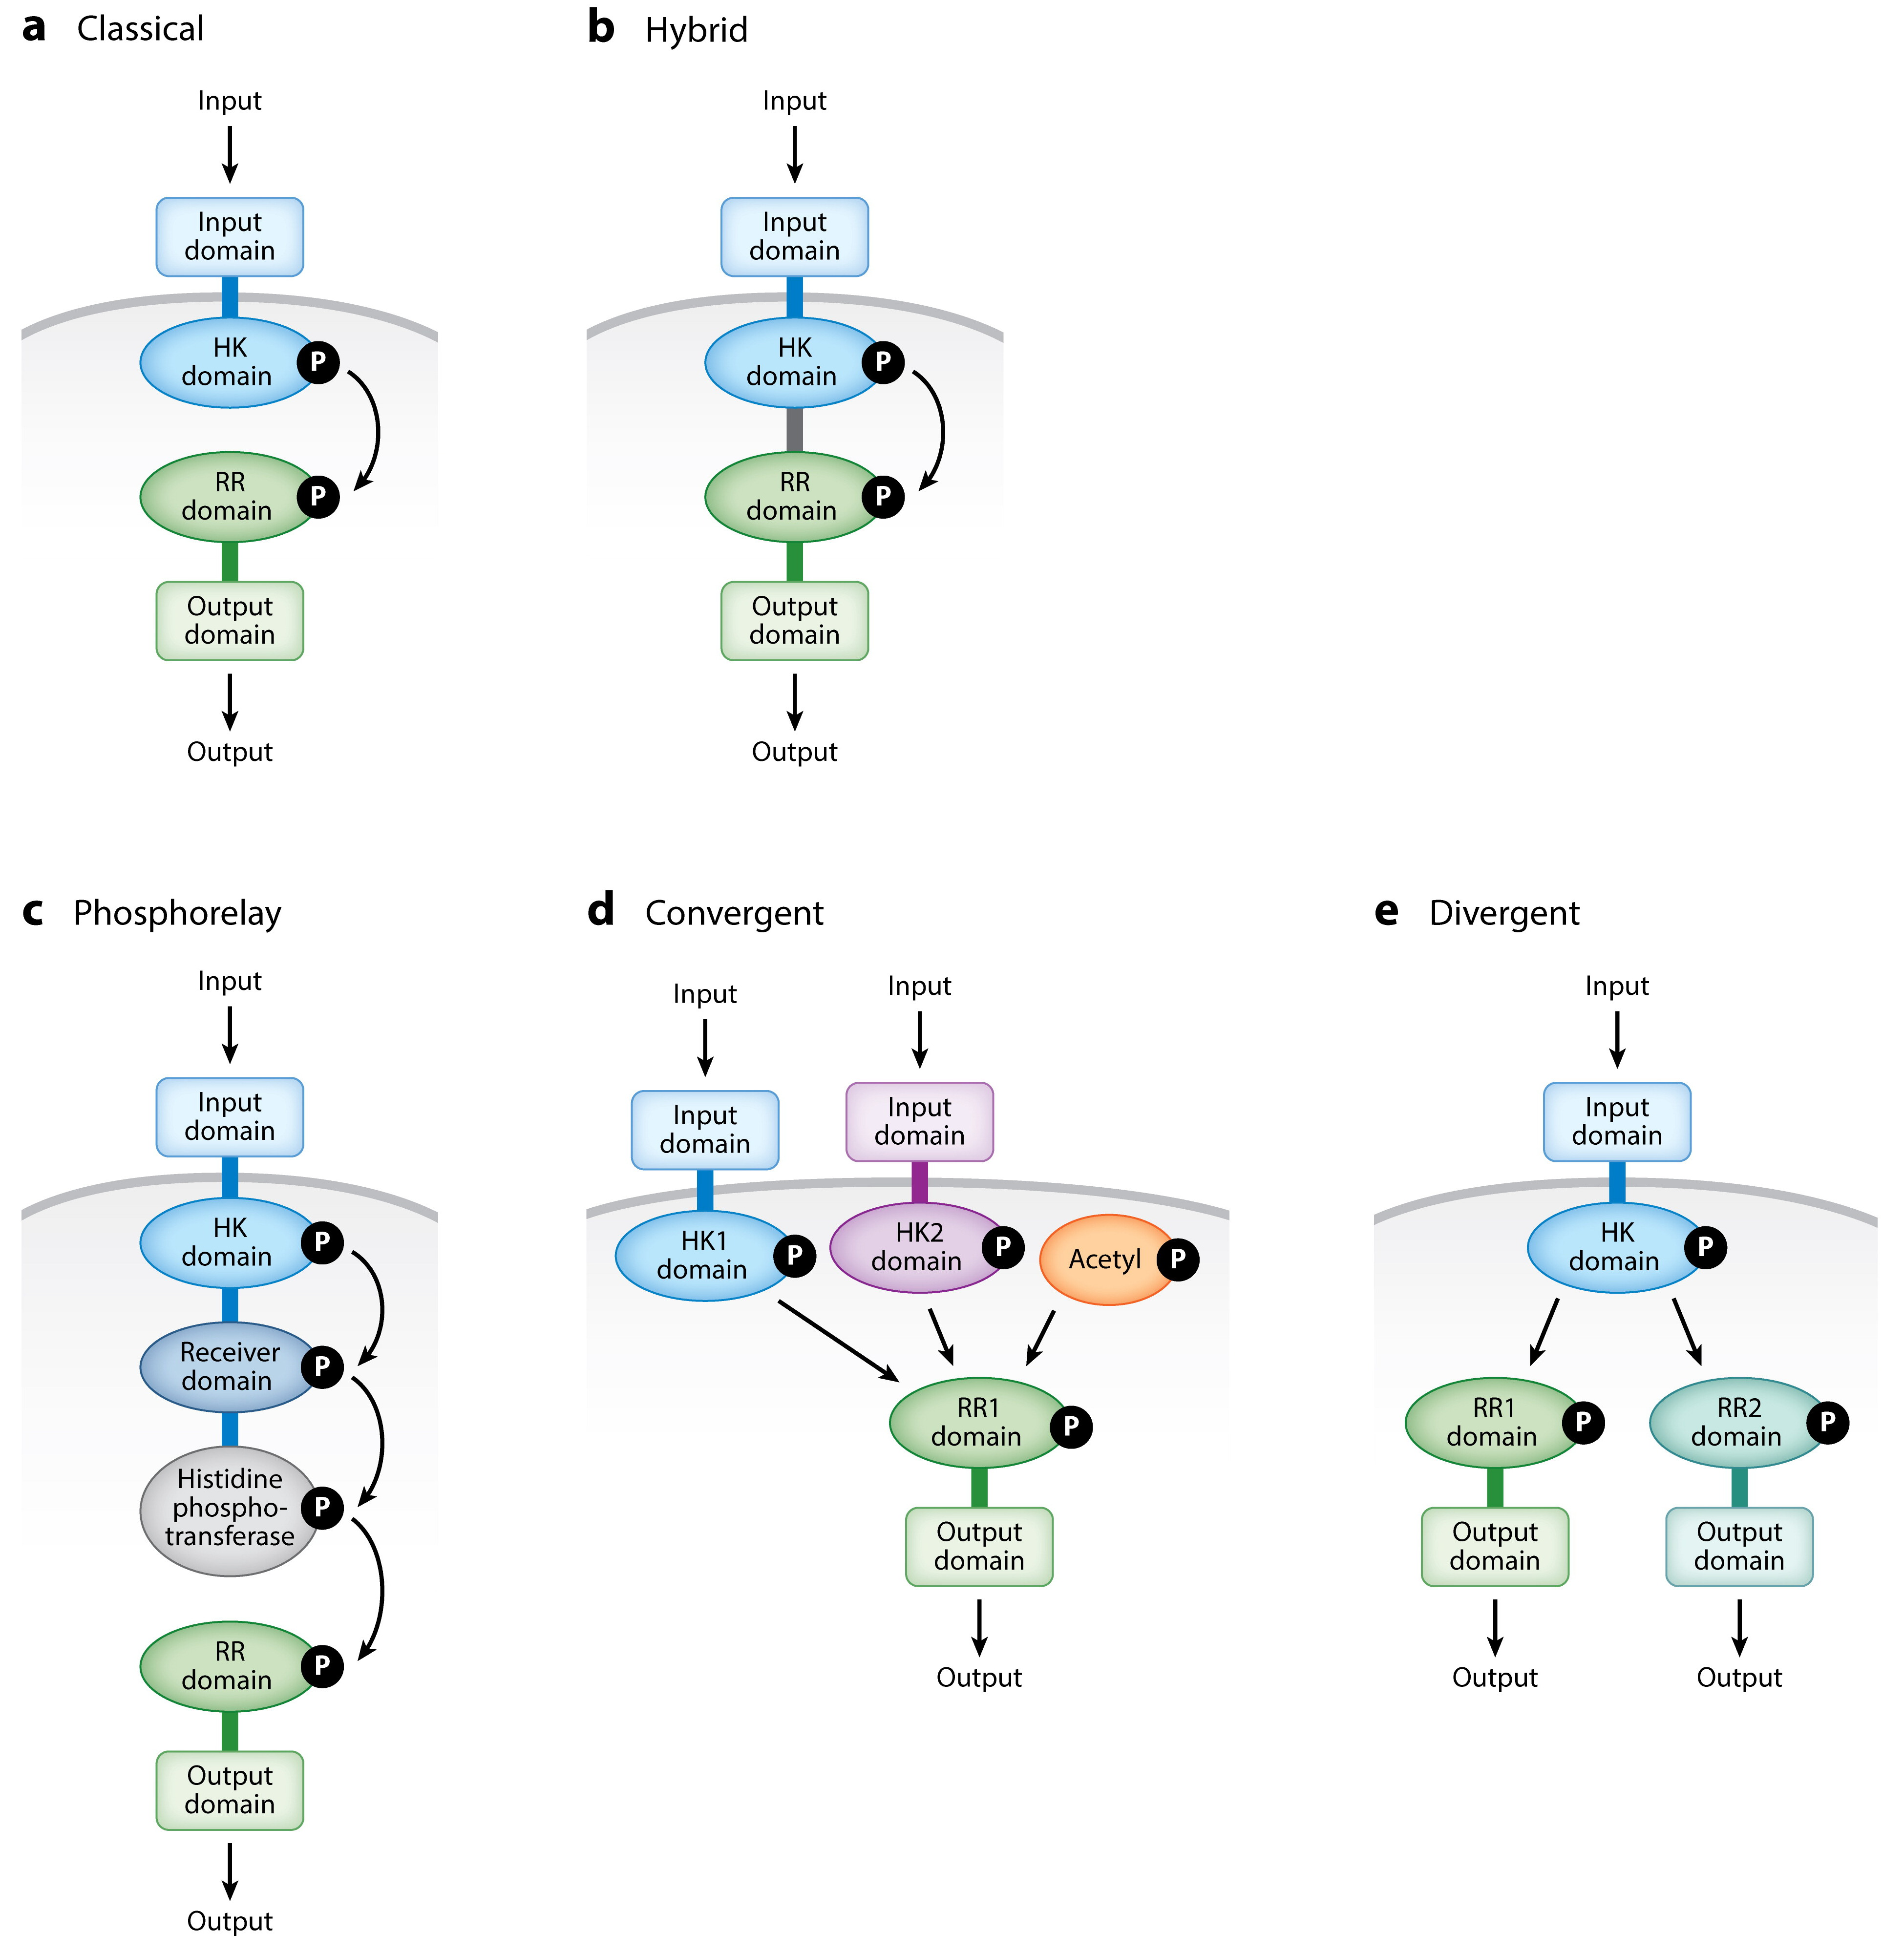
\includegraphics[scale=0.8]{text/Pictures/TwoComponent.jpeg}
    \caption{Two-component signalling pathways; \textbf{a} histidine kinase (HK) autophosphorylates in response to a signal and subsequently transfers the phosphate to a response regulator (RR) which generates an output; \textbf{b} a hybrid system comprises both components (HK and RR) into a single protein; \textbf{c} in phosphorelay the phosphate is transferred multiple times before reaching its final RR; \textbf{d} some RR can be activated by several HK including metabolites such as acetyl phosphate; \textbf{e} one HK might phosphorylate multiple RR generating various outputs. (reproduced from \cite{groisman2016feedback})}
    \label{two}
\end{figure}

A classic example of indirect signalling is the two-component system.
This consists of a transmembrane sensory kinase which is autophosphorylated at its histidine residue after receiving a signal from the environment (Fig. \ref{two}\textcolor{red}{a}).
To be able to phosphorylate itself the kinase requires ATP or other phosphate donors.
Next, the phosphorylated kinase transfers the phosphate group to its partner regulatory protein enabling its activity, most often DNA-binding and transcriptional regulation \cite{lynch2012prioritization, gao2015temporal, cui2018novel}.
This protein receives the phosphate to its aspartate residue and might act as both gene repressor and/or activator.
Alternatively, the regulatory protein can modify biochemical activity of target proteins or RNAs instead or on the top of the change in gene expression \cite{shu2002antar, chambonnier2016hybrid}.
Hybrid two-component systems also exist, and are usually located in the cell membrane with their sensory domains in periplasmic space (Fig. \ref{two}\textcolor{red}{b}) \cite{lynch2012prioritization, hirano2013regulon}.

Another version of two-component system is the phosphorelay (Fig. \ref{two}\textcolor{red}{c}).
In this case, multiple steps of phosphate transfers occur before the final phosphorylation of target regulator.
These multiple steps allow for easier regulation by other signals as the phosphorelay can be silenced at any of the intermediate steps during the transmission \cite{perego2001pentapeptide, groisman2016feedback}.

In some cases, multiple different signals are detected by the same sensory kinase or converge into the same regulatory protein (Fig. \ref{two}\textcolor{red}{d}).
This results in similar outputs in response to various signals \cite{kaczmarczyk2014complex, chambonnier2016hybrid}.
In contrast, a divergent signal transmission results in multiple responses to the same signal (Fig. \ref{two}\textcolor{red}{e}) as one sensory kinase is able to phosphorylate aspartate domains of different acceptor proteins \cite{mika2005two, groisman2016feedback}.

\section{Signal processing}
After a signal is received by the cell, it triggers changes in the activity of proteins and/or gene expression.
Control of protein activity helps to respond to rapid environmental changes. Translational regulation is a useful tool for controlling the differential production of proteins coded within the same operon and thus transcribed on the same mRNA \cite{dar2018extensive}.
Transcriptional regulation might be considered as the most economical response as it inhibits the synthesis of products which are not needed at the moment.
This saves resources and energy for synthesis of desired gene outputs.
As the latter type of regulation is the focus of this work, I outline the important aspects of this process in more detail below.

\subsection{Regulation of transcription initiation}
Initiation of transcription is the first step of gene expression and as that it is highly regulated.
The crucial step is RNA polymerase binding to the promoter sequence, which contains motifs known as: the -35 element, the extended -10 element, the -10 element, the
discriminator region, the UP element and the core recognition element.
These elements mediate the interaction of the promoter and RNA polymerase, and their proximity to consensus sequences influences the strength of the promoter.
The rate of transcription initiation is proportional to the total amount of produced mRNA as long as an early transcription termination does not occur \cite{kennell1977transcription, iyer1996absolute}.
Here I am going to describe the regulation of this step involving transcription factors.
The activity of these factors corresponds to signals the cell acquires from the internal or external environment.
Even though some factors control only one promoter, the majority of at least \tax{E. coli} promoters is regulated by more transcription factors \cite{karp2014ecocyc}.

\begin{figure}[ht!]
  \centering
  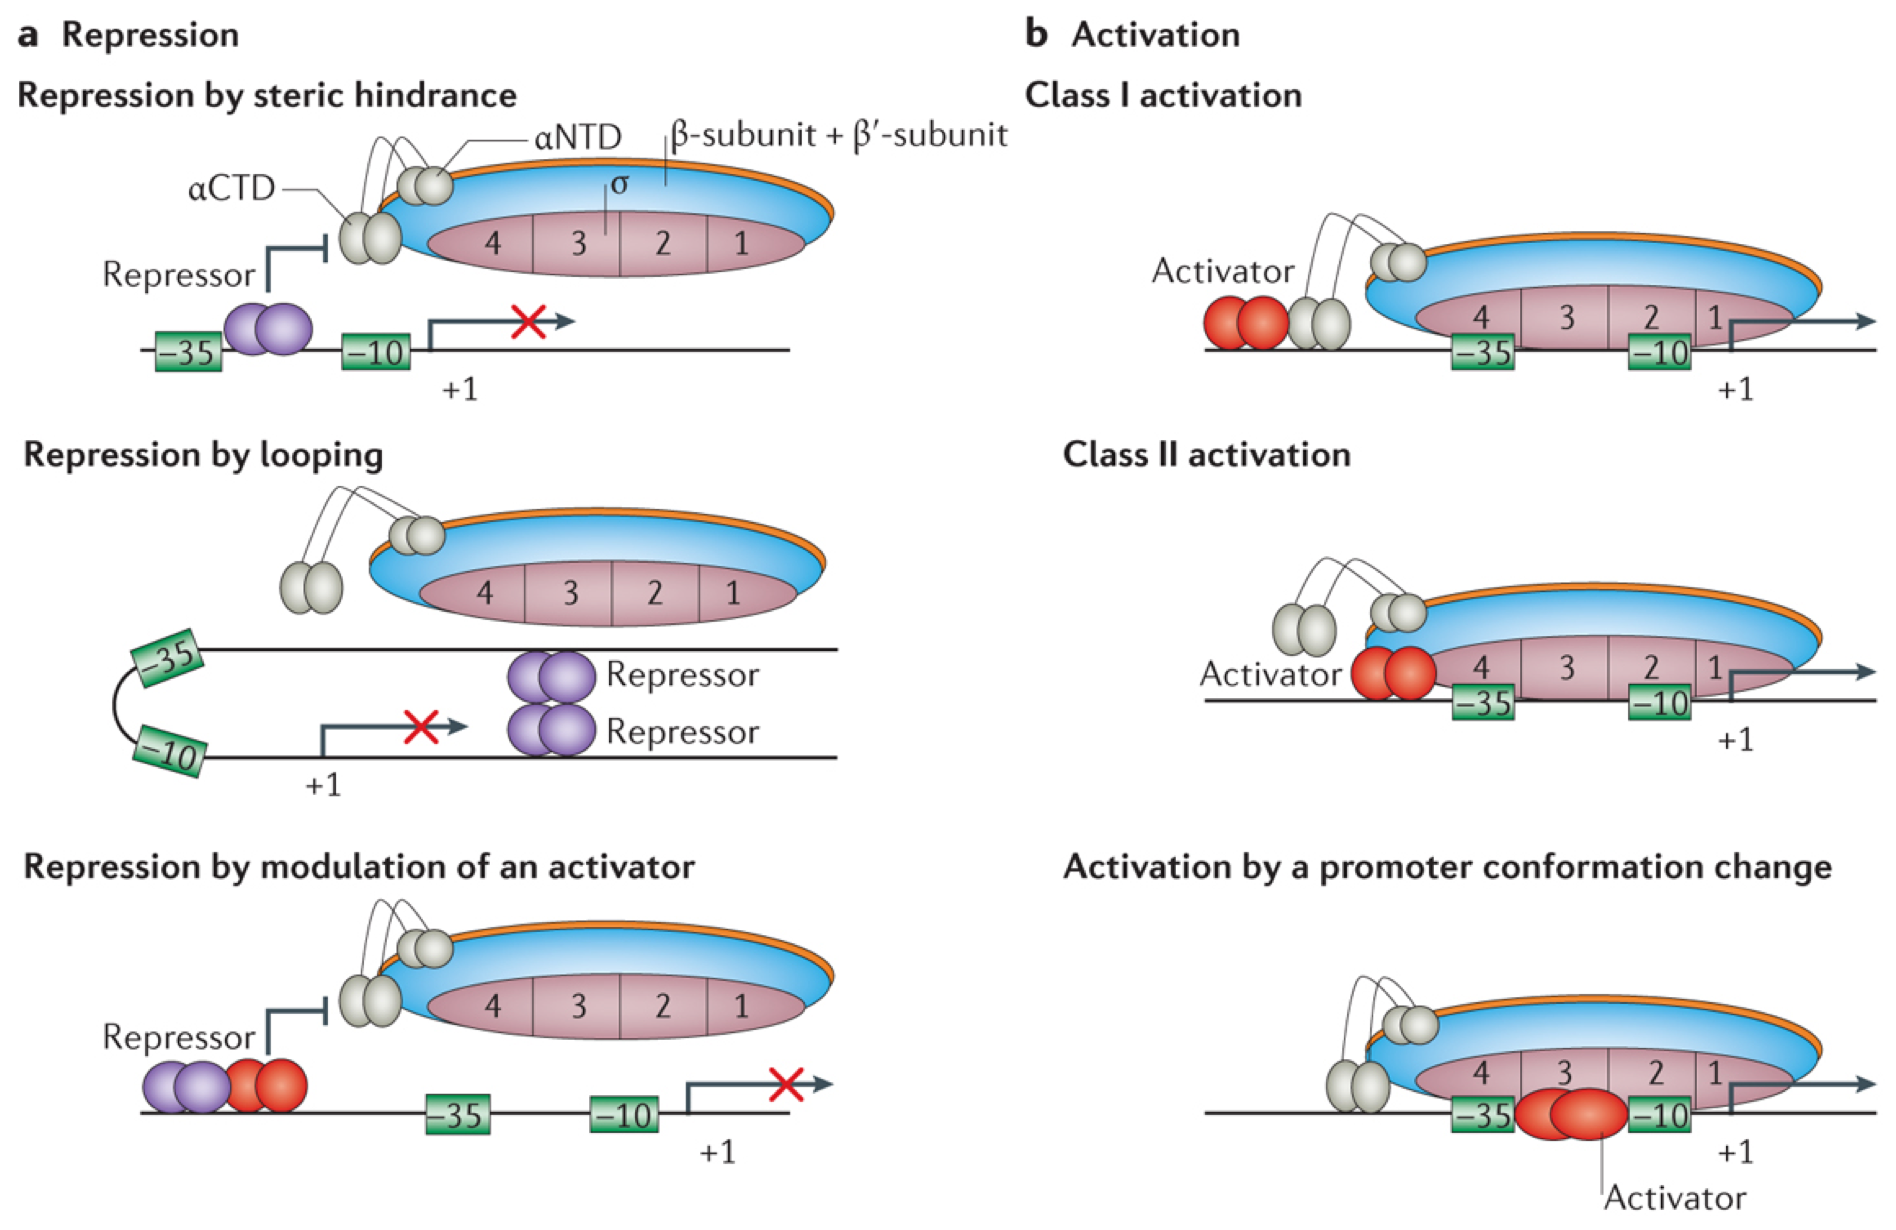
\includegraphics[scale=0.4]{text/Pictures/TxnInitRegulation.png}
    \caption{Regulation of transcription initiation by repressors and activators. (reproduced from \cite{browning2016local})}
    \label{txn}
\end{figure}

\subsubsection{Repression}
Repression of promoters is often based on producing an obstacle in the place of -10 and -35 elements which blocks RNA polymerase binding to the promoter.
This is achieved through various mechanisms.
The simplest one is repressor binding to the operator which overlaps one or both of those promoter elements \cite{brent1981mechanism} (Fig.~\ref{txn}\textcolor{red}{a}).
Other promoters have distant operators outside -10 and -35 elements, but bound repressors cluster creating a DNA loop which also constitutes a blockage \cite{semsey2004dna} (Fig.~\ref{txn}\textcolor{red}{a}).
A more complex and indirect way of repression is by inhibiting activators (described below) - i.e., repressors acting as anti-activators \cite{sogaard1993protein}.
Because some promoters require activation for transcription initiation, anti-activation might be sufficient for complete repression (Fig.~\ref{txn}\textcolor{red}{a}).

The activity of specific promoters can be controlled gradually.
Such promoter sequences have arrays of operators, and the amount of bound repressors affects the strength of the repression.
Alternatively, some promoters can be recognized by multiple repressors which usually do not affect each other \cite{el2009repression}.

For instance, arginine acts as a co-repressor of its own biosynthesis (Fig. \ref{dir}\textcolor{red}{a}).
When a bacterium does not have enough of this amino acid available for protein production the transcription of arginine genes is active \cite{charlier2004biosynthesis, caldara2006arginine}.
On the other hand, when arginine is abundant in the culture medium, and thus in the cell, there is no need to make more of it.
The cell has ArgR repressor present in the cytosol, but ArgR itself cannot bind to DNA and inhibit transcription in the absence of arginine \cite{clark2005molecular, caldara2006arginine}.
However when there is plenty of arginine in the cell, it binds to ArgR and as a co-repressor inhibits expression of arginine structural genes by binding to an appropriate promoter \cite{charlier1992arginine, charlier2004biosynthesis, clark2005molecular}.

\begin{figure}[ht]
  \centering
  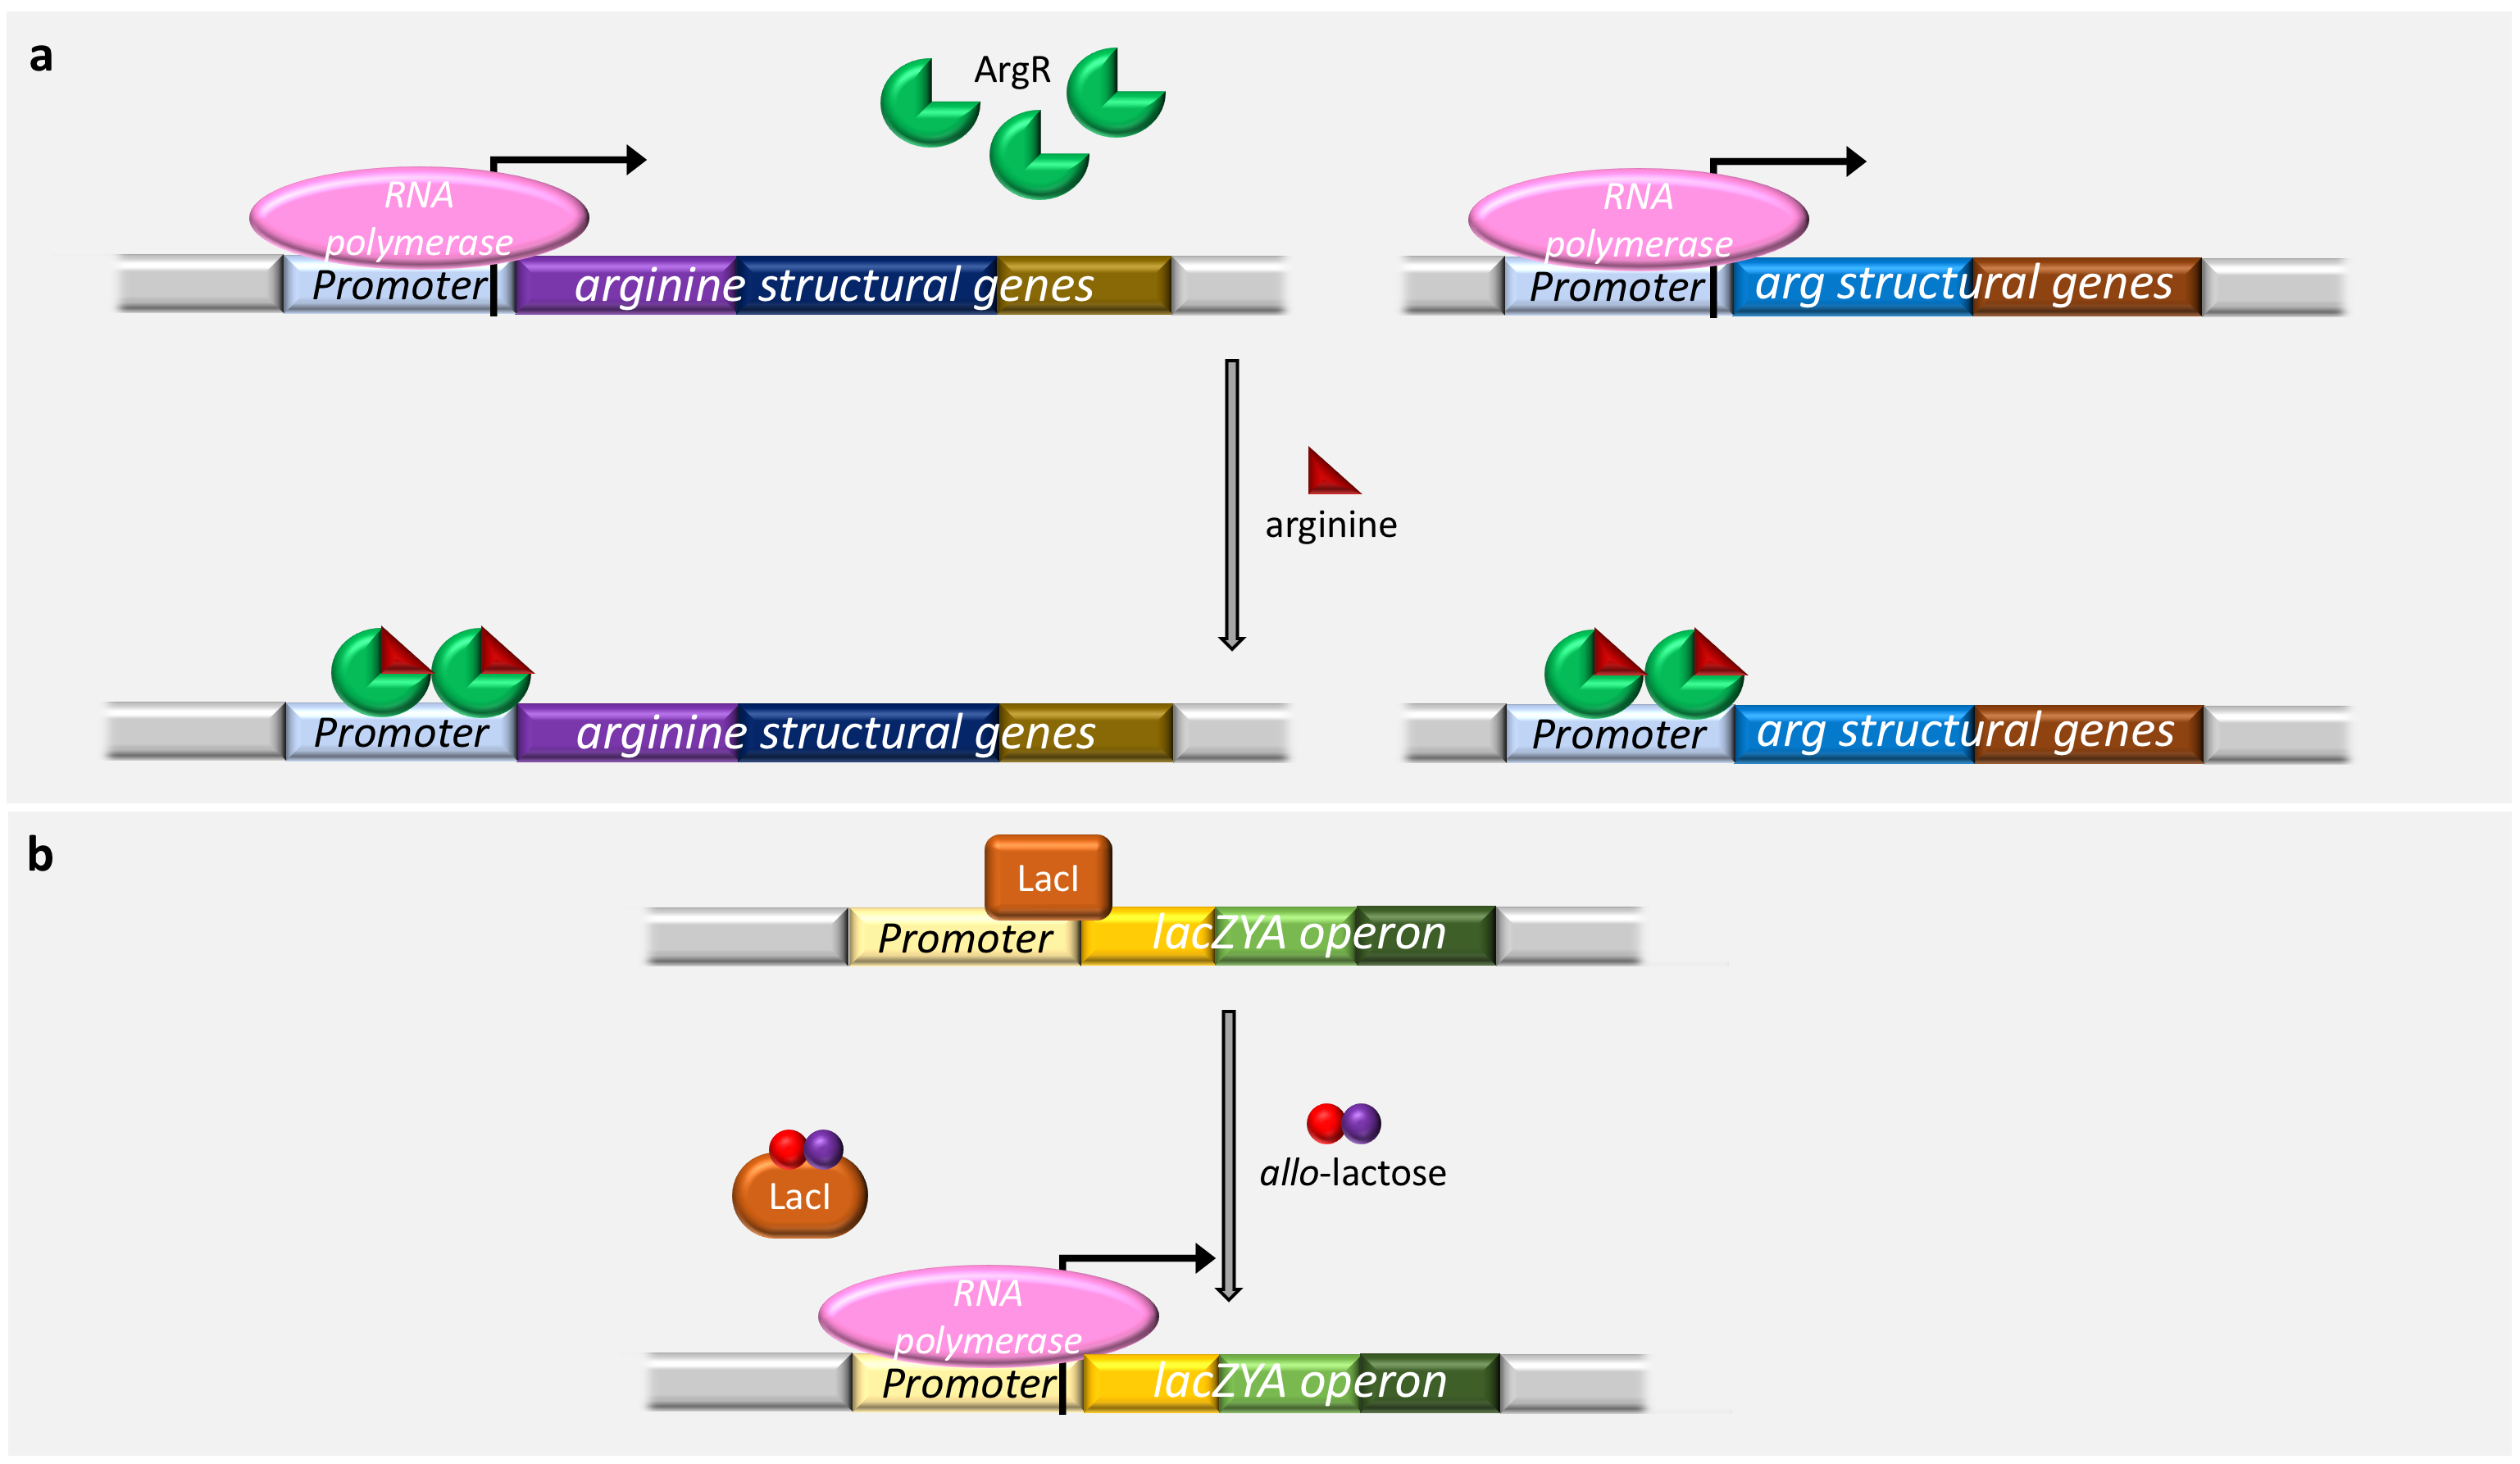
\includegraphics[scale=0.27]{text/Pictures/DirectSignaling.png}
    \caption{Scheme of repression and activation; \textbf{a} expression of arginine structural genes is co-repressed by arginine itself, because without it ArgR repressor cannot bind to the DNA; \textbf{b} if \tax{lac} operon anti-repressor (allolactose) is present it binds to LacI repressor and induces \tax{lac} operon transcription.}
    \label{dir}
\end{figure}

\subsubsection{Activation}
Activation enables particular gene transcription or increases the strength of RNA polymerase binding to the promoter.
Similar to repression, some activators interact directly with RNA polymerase but others act indirectly as anti-repressors most often by releasing bound repressors and preventing their further binding to the operator \cite{frederix2011co}.
Besides affecting sequence specific repressors, some indirect activators also affect binding of nucleoid-associated proteins (NAPs; described more in the next section), altering access for RNA polymerase to the promoter sequence \cite{santana2001transcriptional}.
Direct activators mostly facilitate the interaction of RNA polymerase and promoter.
Three mechanisms of direct activation are usually described: class I activation, class II activation, and activation by conformational change.

Class I activators bind upstream of -35 element and interact with the $\alpha$ subunit of RNA polymerase \cite{ushida1990helical} (Fig.~\ref{txn}\textcolor{red}{b}).
Operators of class II activators in turn overlap with -35 promoter element and the activators interact with a given $\sigma$ factor of RNA polymerase \cite{igarashi1991functional} (Fig.~\ref{txn}\textcolor{red}{b}).
Moreover, bound class II activators prevent binding of the RNA polymerase $\alpha$ subunit to the preferred position right upstream of -35 element.
Class I and class II activation thus can co-occur on the same promoter when two different activators are required to trigger the transcription \cite{lloyd2002requirement}.

The last classical activation mechanism causes a conformational change of the sequence between -10 and -35 elements.
RNA polymerase binding to these promoters without an activator is weakened or impaired due to an inappropriate distance between -10 and -35 elements.
This is also where the operators of such activators are located (Fig.~\ref{txn}\textcolor{red}{b}).
A bound activator then brings the elements into the optimal position for RNA polymerase recruitment \cite{heldwein2001crystal}.

% 17.9.2018
% this is a lot of detail on s54, not sure it's needed.
%%%All activation mechanisms mentioned above just enable RNA polymerase binding strong enough for efficient transcription initiation.
%%%Other kind of activation of transcription initiation is not even required for most RNA polymerase holoenzymes.
%%%However, RNA polymerase containing $\sigma^{54}$ factor is unable to unwind promoter DNA to begin transcribe.
%%%This is facilitated by enhancer binding proteins (EBPs) which interact with the $\sigma^{54}$ factor \cite{morett1989vivo, cannon2000dna}.
%%%Nevertheless, EBPs bind upstream of the promoter elements, so to get in contact with the $\sigma^{54}$ factor a loop has to be produced.
%%%Production of this loop is known to be mediated by nucleoid-associated protein IHF which as well as other NAPs plays a role in DNA accessibility \cite{de1991upstream, sze2001vivo}.

Gene activation is best studied in the \tax{lac} operon of model organism \tax{E. coli}.
To avoid wasteful production of the enzyme hydrolysing lactose (LacZ), if no lactose is available, \tax{E. coli} expresses \tax{lac} repressor (LacI) \cite{hudson1990co}.
However, \tax{lac} operon transcription is desired if lactose is present in the media, and this is ensured by \tax{lac} operon inducers.
Allolactose - \tax{lac} operon inducer - is imported by lactose permease into the cell where it binds directly to the repressor LacI.
Lactose has to be modified to allolactose by $\beta$-galactosidase (LacZ) to act as a \tax{lac} operon inducer \cite{jobe1972lac, wheatley2013structural}.
Allolactose then induces \tax{lac} operon gene indirectly by acting as an anti-repressor.
LacI binding to the promoter DNA is then released triggering \tax{lacZYA} expression (Fig. \ref{dir}\textcolor{red}{b}) together with binding of general regulatory protein CRP \cite{hudson1990co, clark2005molecular}.
CRP levels rise when the availability of a preferred carbon source (e.g., glucose) drops.
Low levels of CRP thus prevent lactose utilization favouring glucose consumption even when lactose is available.

\subsection{Regulation of mRNA elongation and transcription termination}
After a successful transcription initiation, the elongation of mRNA follows until termination occurs.
Even though the main transcription regulation occurs at the level of transcription initiation, elongation and termination can also be modulated, ranging from the repression of elongation \cite{monsalve1996protein}, through elongation pausing and backtracking \cite{mustaev2017transcription} to transcription attenuation and anti-termination \cite{naville2009transcription}.

\subsection{Transcription network topology}
For a better understanding of the whole transcription network regulation, it is important to look at how individual transcriptional motifs affect the speed of regulatory circuits, transcriptional noise, and possible epigenetic memory.
The speed in transcriptional response is usually characterised by a rise-time (or response time), i.e., a time when the concentration of a gene product reaches its half maximal concentration after gene induction.
While the effects of different signal sensing mechanisms (described above) on the transcriptional response dynamics (e.g., speed, noise, sensitivity) are not well studied, the ways in which network motifs affect these aspects are better understood.

\phantomsection%%% removes warning: "package hyperref warning the anchor of a bookmark and its parent's must not be the same. Added a new anchor on input line 172."
\subsubsection{Promoter strength and protein lifetime}
The stronger a promoter the more easily and often RNA polymerase binds to it and the more of an appropriate protein is produced at the time.
The strength of the promoter is given by its nucleotide sequence and binding of transcription factors increases or decreases RNA polymerase affinity to it.
On the other side of this equilibrium is the degradation of the product, as its stability in certain conditions determines its lifetime.
A functional protein is also diluted during cell division, which further reduces its concentration in a cell.

%%%\subsubsection{Transcriptional network motifs}
\subsubsection{Feedback loops}
A feedback loop is a transcriptional network motif in which the products affect their own production (Fig.~\ref{motifs}\textcolor{red}{a},\textcolor{red}{b}).
The influence of the output on its own transcription might be direct or indirect if multiple effectors are involved.
Feedback loops are quite common in bacterial gene regulation and affect the speed, variation, and sensitivity of cellular responses and can also lead to epigenetic switches.
First, the effects of feedback loops on transcription dynamics are characterized below, further a relationship between these loops and cell memory is described.
Note that most of the work on feedback loop dynamics has been done by comparing the feedback loops to systems with no feedback, and not by positive versus negative feedback comparison.

A positive feedback loop is a motif in which the product further induces the expression of the gene coding it (Fig.~\ref{motifs}\textcolor{red}{a}).
Transcriptional activation is slower and noisier in case of positive feedback loops compared to no feedback systems \cite{maeda2006regulatory, sayut2007noise}.
This is probably due to low initial amounts of the auto-inducer which might either be diluted before the expression is fully auto-induced or are bound to other functions within the cell.
This stochasticity in auto-inducer binding to its promoter is likely to cause higher transcription noise upon the induction among individuals and delay the effect of the strong induction by positive feedback.
Although slower and noisier, this motif enables cells to react to much lower concentrations of a signal once the positive feedback loop establishes.
Both graded and hysteretic expression (i.e., ON or OFF expression state depending on recent events or memory) can occur in genes regulated this way \cite{maeda2006regulatory}.

A negative feedback loop, i.e., a circuit where the product inhibits its own expression, exhibits the opposite traits of a positive feedback, as it decreases the response time \cite{rosenfeld2002negative} (Fig.~\ref{motifs}\textcolor{red}{b}).
It also reduces the variability in product concentration decreasing cell-to-cell and temporal variability \cite{becskei2000engineering}.
This enables the cell to use stronger promoters for proteins needed in a short time but at low concentration without overshoots and risks of protein toxicity.
Hysteresis in terms of simple negative feedback loop has not been reported but could be readily achieved by double-negative feedback \cite{toman1985system}.
An example of this is detailed below.

Positive feedback loops and double-negative feedback loops are known to play a role in memory of bacteria.
Positive feedback is the first described example of bacterial epigenetics.
It was shown in 1957 that an \tax{E. coli} sub-population primed by high concentration of lactose analogue TMG is able to maintain \tax{lac} operon fully induced even in low non-inducible TMG concentrations \cite{novick1957enzyme}.
While if the same bacteria are exposed to the low non-inducible TMG concentration without priming the \tax{lac} operon remains repressed by LacI.
The mechanism behind this resides in different levels of $\beta$-galactoside permease (LacY) present in TMG induced and naive cells.
The induced population has a high level of the permease in the cell membrane, because \tax{lacY} gene expression has been activated by previous high TMG concentrations.
This state is preserved in a sub-population of induced cells after transfer into low TMG concentration as the abundant permease is able to maintain the intracellular TMG level high enough to avoid LacI repression.
Thus the high level of permease leads to high intracellular TMG concentration which in turn acts as permease transcription activator.
On the other side, naive cells have minimal amounts of LacY if any, so they are not able to obtain enough TMG from the solution to activate \tax{lac} operon expression \cite{smits2006phenotypic, casadesus2013programmed}.

\begin{figure}[ht!]
  \centering
  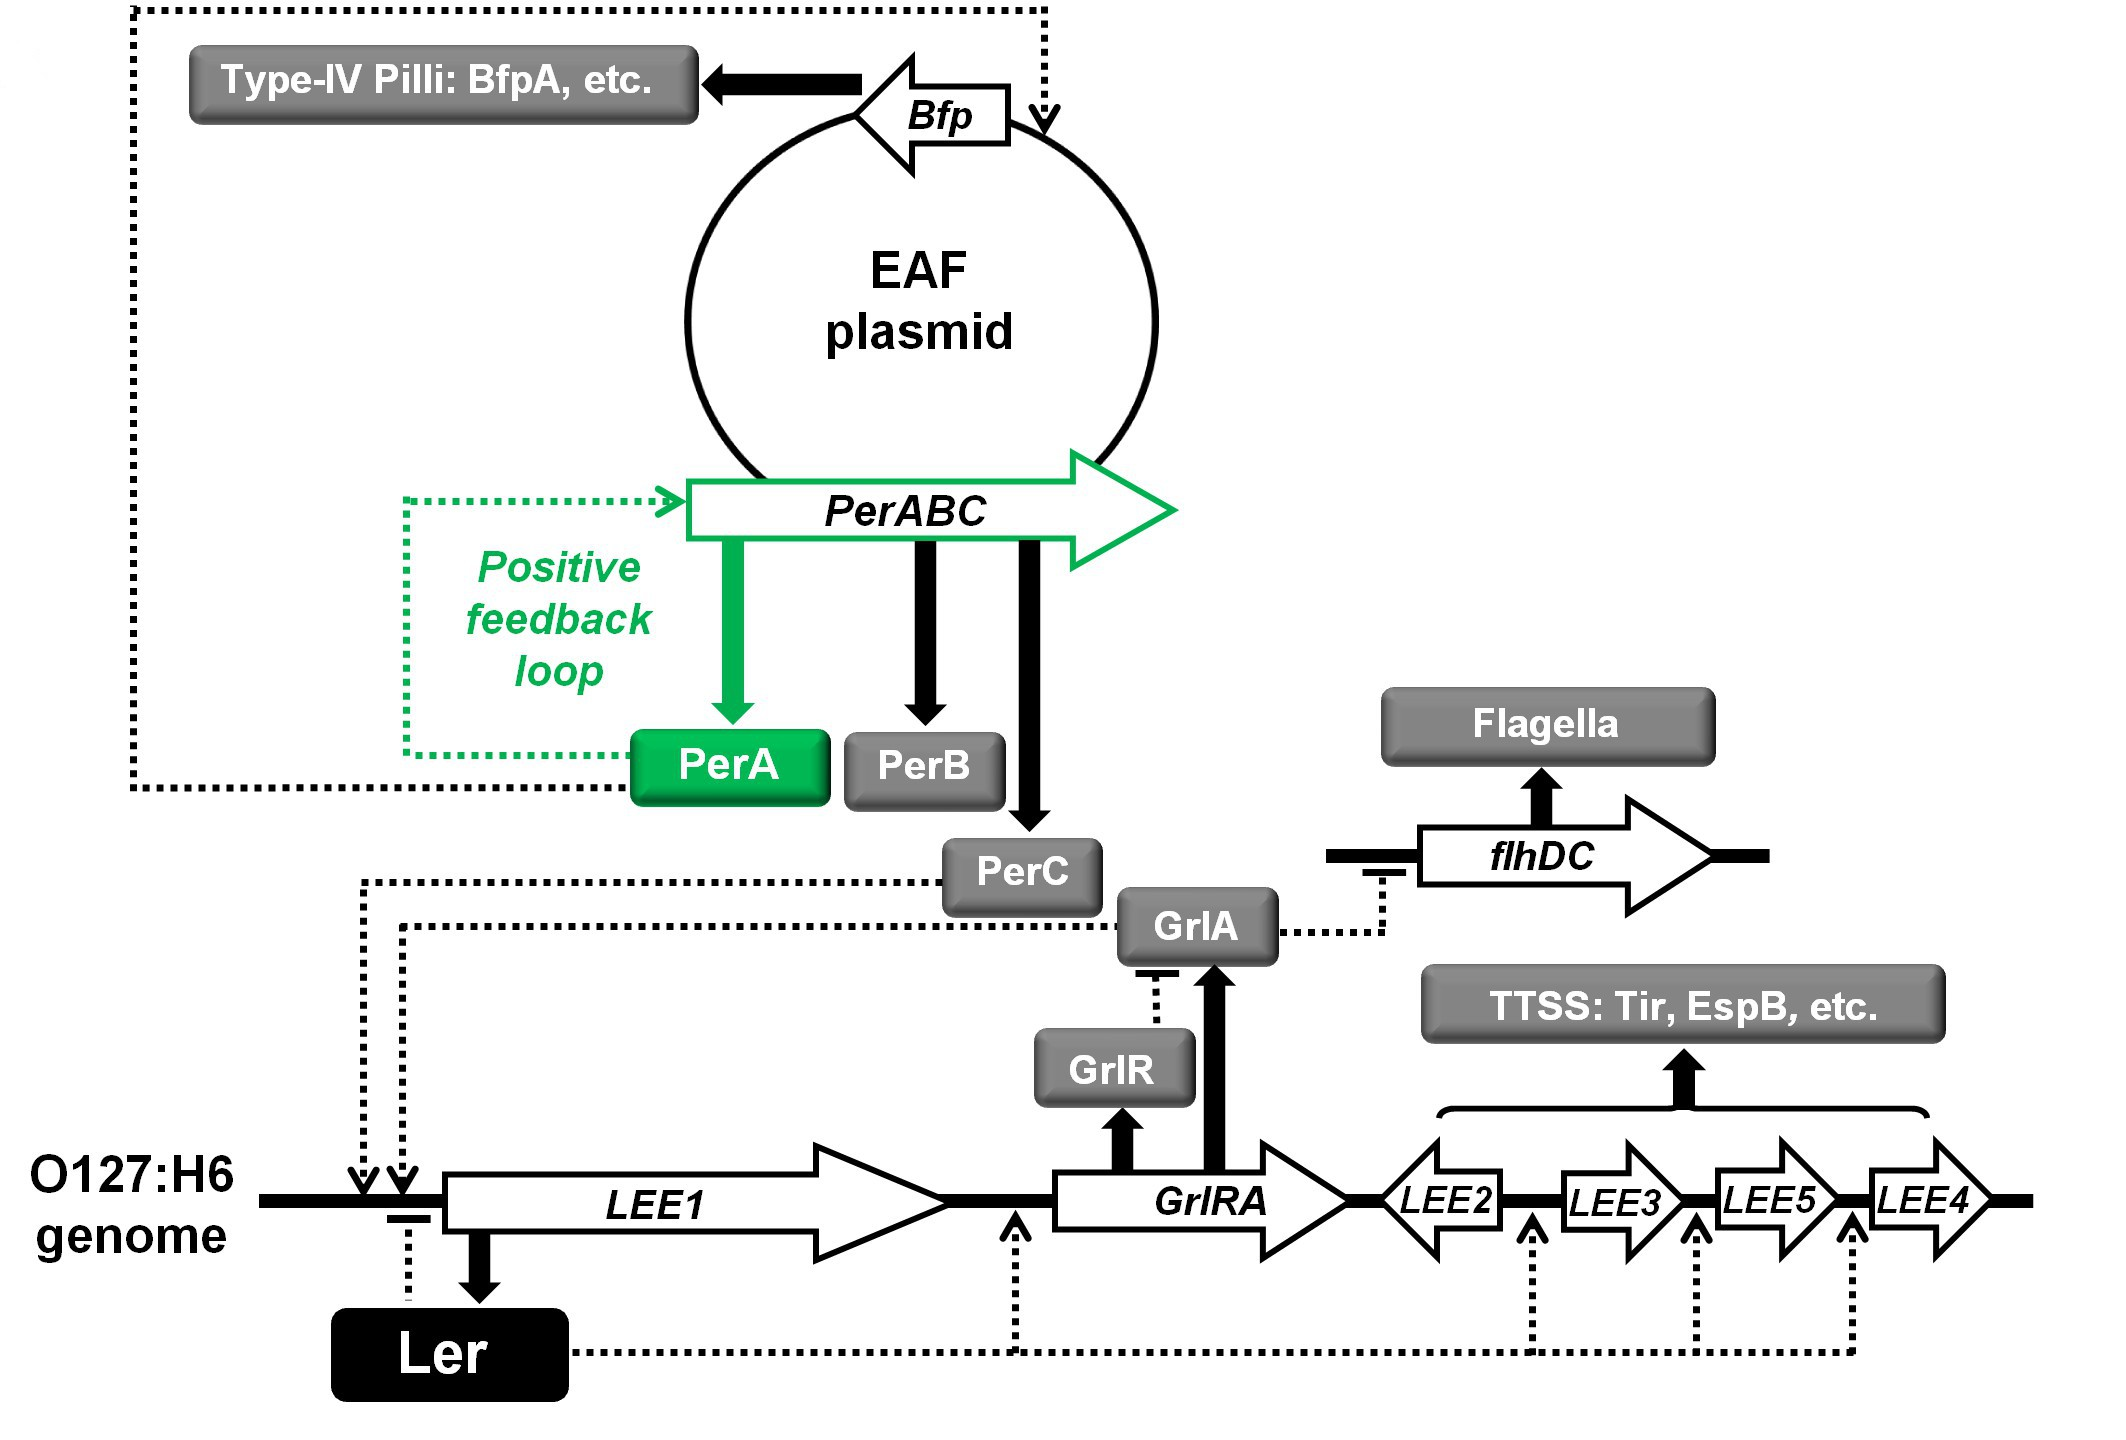
\includegraphics[scale=0.2]{text/Pictures/perOperonRegulation.jpg}
    \caption{Scheme of EPEC virulence regulation. PerA positivelly autoregulates \tax{perABC} operon and triggers expression of type IV pili. PerC activates transcription of Ler which is the main regulator of T3SS secretion system machinery. (reproduced from \cite{ronin2017long})}
    \label{per}
\end{figure}

Another example of a long-term epigenetic switch mediated by a positive feedback loop was published recently.
Enteropathogenic \tax{E. coli} (EPEC) has been revealed to coexists in two, non-virulent and hyper-virulent, sub-populations, each having lag phases of different length \cite{ronin2017long}.
At the transcriptional level it is a change in \tax{per} operon expression (located on EAF plasmid) and \tax{per} regulated genes.
EPEC cultivation in virulence-activating conditions gives rise to \tax{per}-ON hyper-virulent aggregative sub-population (SMALL phenotype) reaching nearly 100\% \cite{ronin2017long}.
Interestingly this high ratio of \tax{per}-ON vs. \tax{per}-OFF cells remained for many generations even after transferring the culture back into non-activating conditions, although naive EPEC culture contains only a minority of \tax{per}-ON cells.
Transition back from \tax{per}-ON to \tax{per}-OFF phase is achieved when cells are grown up to stationary phase.
The long-term stability of \tax{per}-ON state relies on a positive feedback of PerA which acts as an activator of its own gene beside \tax{perB} and \tax{perC} in the \tax{per} operon (Fig.~\ref{per}) \cite{ibarra2003identification, ronin2017long}.

A double negative feedback loop is known to play a role in epigenetic switching between a lytic and lysogenic cycle of \tax{E. coli} phage $\lambda$ \cite{smits2006phenotypic, casadesus2013programmed}.
After inserting its DNA, the virus might undergo two different cycles - i.e., either replicate producing new phages and heading for bacterial lysis or integrate its DNA into the bacterial chromosome and persist there within lysogeny.
The fate of the phage lies in two repressors, CI and Cro, each repressing transcription of the other \cite{eisen1970regulation, neubauer1970immunity}.
Both CI and Cro are produced at the beginning of the infection.
If the level of CI reaches a certain threshold and outcompetes Cro, whose activity is suppressed, the phage enters a lysogenic cycle staying dormant in the cell thanks to a CI-\tax{cI} positive feedback loop.
Otherwise, Cro levels rise further inhibiting CI production and establishing phage proliferation with subsequent cell lysis \cite{svenningsen2005role}.
It should be noted that although it is not predictable whether the phage enters the lytic or lysogenic cycle, the ratio of lysed/lysogenized cells depends on the bacterial physiologic situation and other environmental factors as well.
Interestingly, Toman et al. used the CI-Cro system for epigenetic regulation of \tax{gal} operon in \tax{E. coli} \cite{toman1985system}.
%%% it's not epigenetics in E. coli, but in the phage lambda! (except for the engineered system by Toman et al.)

%%%As the CI-Cro regulation is a phage system, the first evidence of bacterial epigenetics driven by a double negative feedback loop was published just 3 years ago.

%%% detection of double negative feedback loop originating in bacteria?
%%% double negative feedback detected in "A Novel Feedback Loop That Controls Bimodal Expression of Genetic Competence" which talks about cell competence
%%% there is no direct evidence for epigenetics playing a role in it, however paper "Agent-based modeling of competence phenotype switching in Bacillus subtilis" suggests it might be so according to their model
%%% especially when in a similar case - bacillus sporulation is it proven in: "Bet-hedging and epigenetic inheritance in bacterial cell development."
%%% Olin also argumented by "An excitable gene regulatory circuit induces transient cellular differentiation," because they say becoming competent is probabilistic in Bacillus

\begin{figure}[ht!]
  \centering
  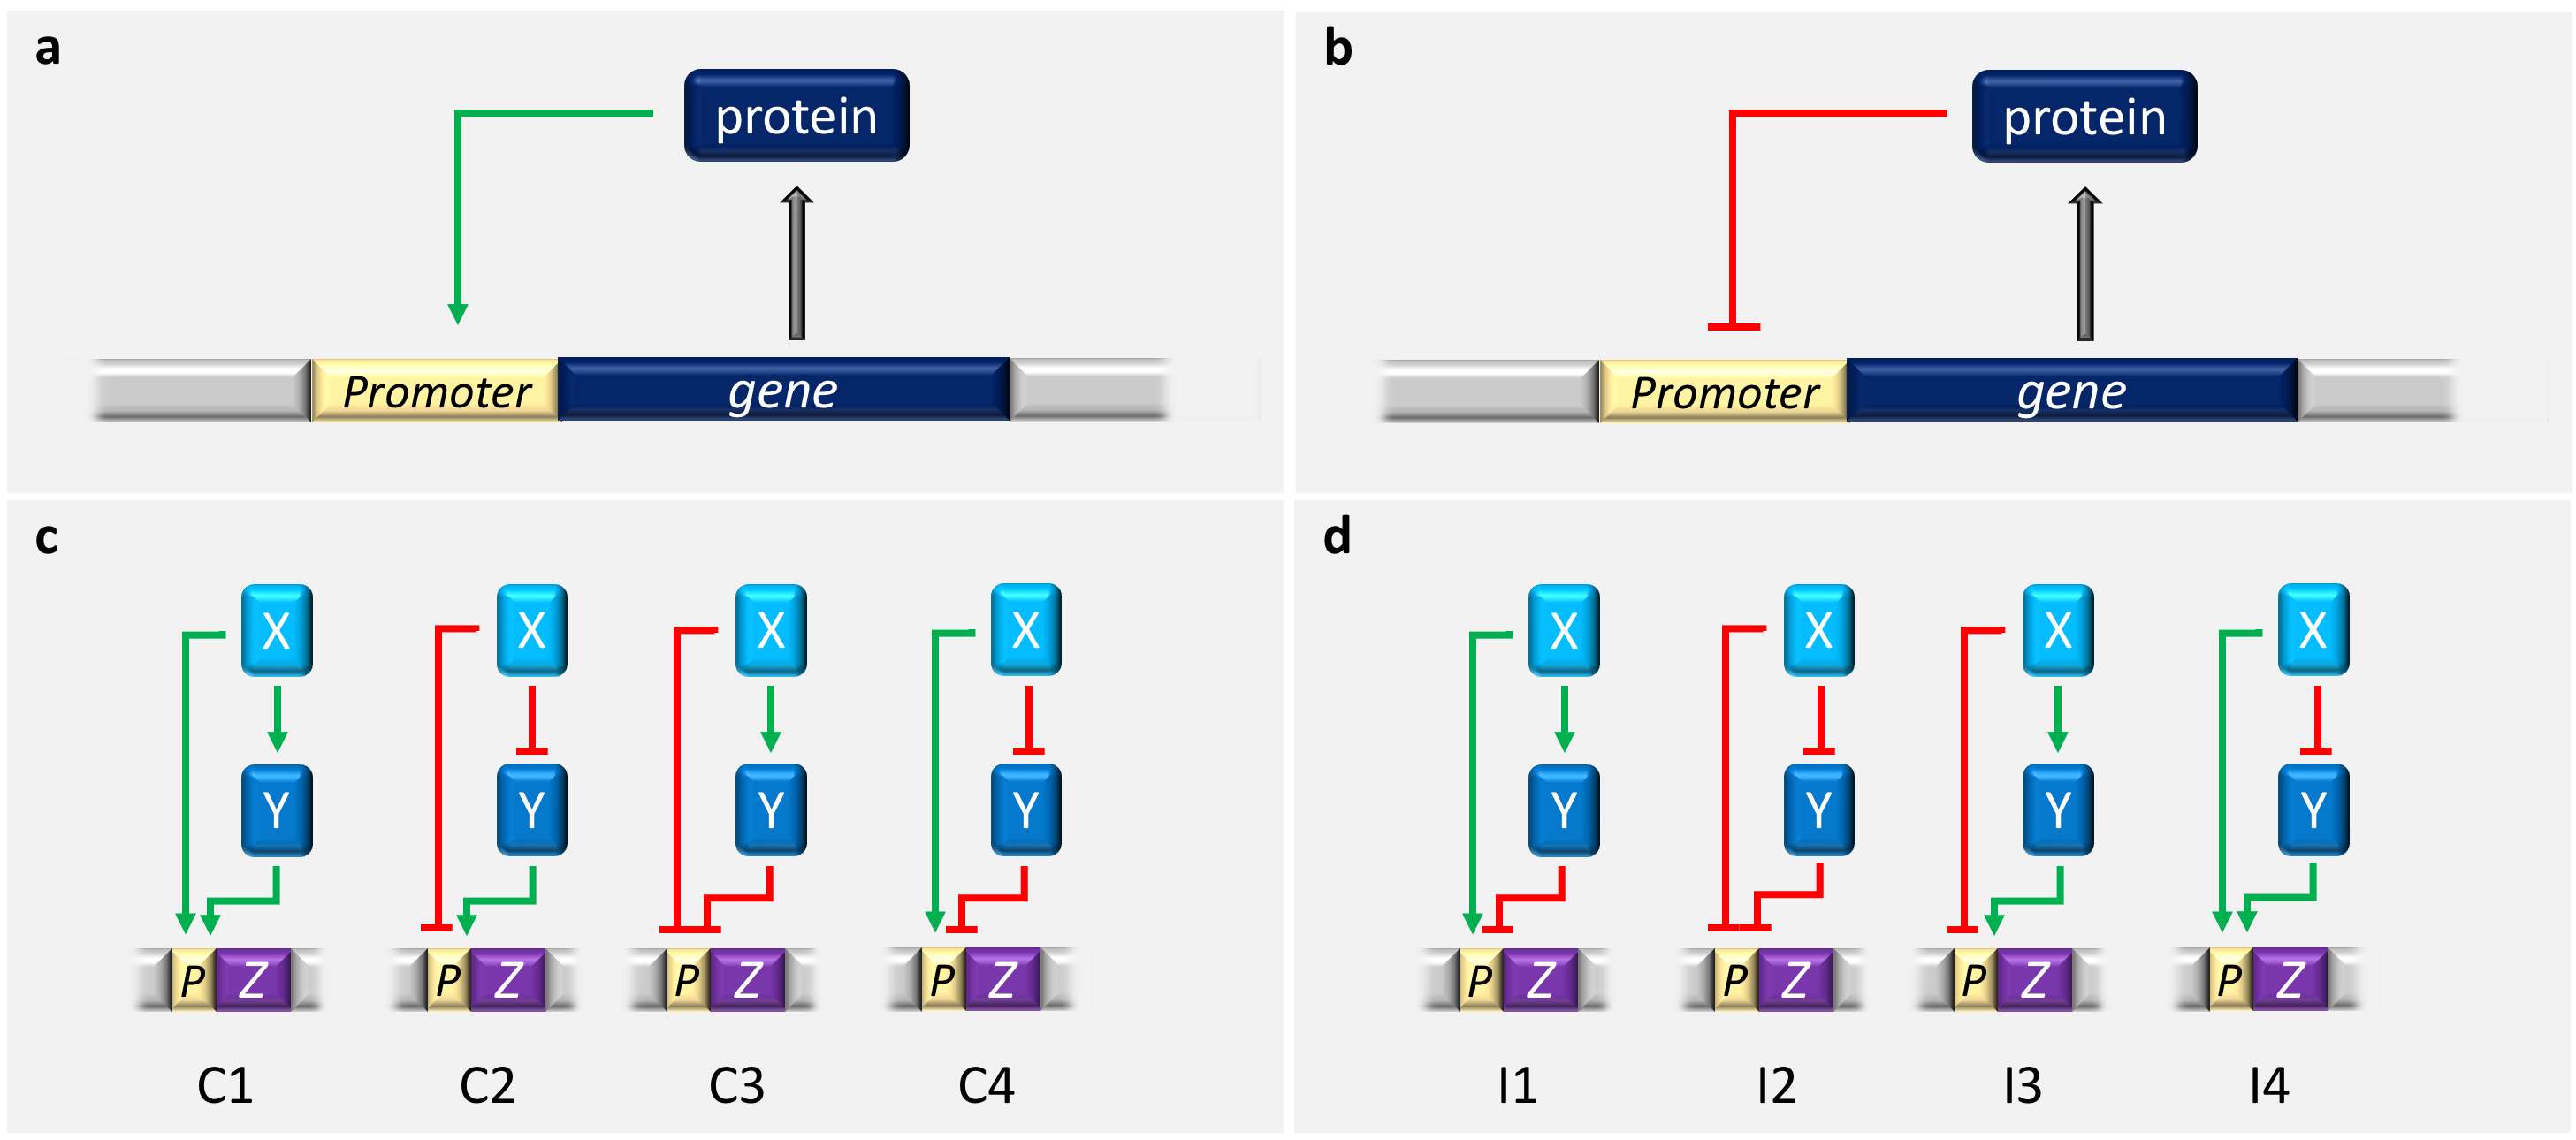
\includegraphics[scale=0.29]{text/Pictures/TxnMotifs.png}
    \caption{Schemes of transcriptional network motifs; \textbf{a} positive feedback loop - gene product induces its own transcription; \textbf{b} negative feedback loop - gene product represses transcription of its own gene; \textbf{c} coherent feed-forward loops; \textbf{d} incoherent feed-forward loops.}
    \label{motifs}
\end{figure}

\subsubsection{Feed forward loops}
Feed forward loops (FFLs) are more complex, but also common regulatory motifs.
A FFL is a regulatory circuit when a transcription factor X regulates another transcription factor, Y, and both (X and Y) regulate a gene or operon Z.
It has been predicted that coherent FFLs  (C1-4; Fig.~\ref{motifs}\textcolor{red}{c}) delay transcriptional responses, while incoherent FFLs  (I1-4; Fig.~\ref{motifs}\textcolor{red}{d}) should act the opposite as transcription accelelators and exhibit transient pulses of expression \cite{mangan2003structure}.
This was later experimentally confirmed, but only in FFL C1 and I1, as these are the most abundant forms shown in Fig.~\ref{motifs}\textcolor{red}{c},\textcolor{red}{d} \cite{mangan2003coherent, kalir2005coherent, mangan2006incoherent}.
The distinction between coherent and incoherent FFL depends on whether the sign (positive or negative) of Z regulation caused by factor X \textit{through} Y is the same as regulation of Z by X itself \cite{shen2002network, mangan2003structure}.
Compared to feedback loops there is little known whether FFLs are involved in any epigenetic mechanism, following text thus covers only their effect on transcriptional dynamics.

Coherent FFL type 1 (Fig.~\ref{motifs}\textcolor{red}{c}, C1), in which both X and Y must bind to trigger transcription (Table \ref{ANDvsOR}; AND-gate logic) delays activation compared to non-FFL systems \cite{mangan2003coherent}.
No delay occurs when transcriptional induction is turned off.
On the other hand, if only factor X or Y is sufficient to induce Z (Table \ref{ANDvsOR}; OR-gate logic in C1 FFL) gene activation is not delayed, but its deactivation is delayed considerably \cite{kalir2005coherent}.
The AND-FFL prevents Z expression when the concentration of X fluctuates close to a threshold, while the OR-FFL enables continuous production of Z even if X concentration drops below a threshold for a while.

\definecolor{mygreen}{RGB}{30,180,0}

\begin{center}
\LTcapwidth=\textwidth
    \begin{longtable}[c]{|c|c|c|c|}
\caption{Relationship among expression activity (ON vs. OFF) in FFL C1, gate logic (AND vs. OR) in regulation and absence or presence (0 vs. 1) of trascription inducers} \label{ANDvsOR} \\

\toprule \multicolumn{1}{|c|}{\textbf{inducer X}} & \multicolumn{1}{c|}{\textbf{inducer Y}}  & \multicolumn{1}{c|}{\textbf{AND-gate logic}} & \multicolumn{1}{c|}{\textbf{OR-gate logic}} \\
\midrule
\endhead

\bottomrule
\endlastfoot

0 & 0 & \textcolor{red}{OFF} & \textcolor{red}{OFF} \\
\hline
0 & 1 & \textcolor{red}{OFF} & \textcolor{mygreen}{ON} \\
\hline
1 & 0 & \textcolor{red}{OFF} & \textcolor{mygreen}{ON} \\
\hline
1 & 1 & \textcolor{mygreen}{ON} & \textcolor{mygreen}{ON} \\
    \end{longtable}
\end{center}


From incoherent FFL motifs, type 1 is predominant in \tax{E. coli} transcriptional network.
Factor X here positively regulates both Y and Z; however factor Y acts as an inhibitor of the Z gene (Fig.~\ref{motifs}\textcolor{red}{d}, I1).
This incoherent FFL speeds up transcriptional responses and was used to create effective transcriptional pulses (or transcriptional bursting), although weak pulse-generating was expected \cite{mangan2003structure, basu2004spatiotemporal, mangan2006incoherent}.
The acceleration trait was confirmed despite the fact that other motifs (e.g., feedback loop) contributed to the used regulatory system.
This suggests that the motifs' fundamental functions are preserved even when combined with other motifs.
Overall this type of regulation similarly, to negative feedback loop shortens the rise-time, but unlike the negative feedback does not avoid overshoots rather the opposite.
The overshoot is seen as a pulse of high gene Z expression which is subsequently inhibited by factor Y, but not necessarily back to the basal level.

\section{Global control of transcription}
Differential physical access to DNA within a chromosome presents one of the explanations to observed variations in promoters activity based on their position in the chromosome \cite{bryant2014chromosome}.
Nucleoid-associated proteins (NAPs) and supercoiling are general mechanisms affecting this accessibility.
NAPs' role in several cellular processes such as replication, horizontal gene transfer or transcription regulation was shown \cite{dixon1984protein, kayoko1992histone, aznar2013hha}.
Here I mention their global influence of gene expression and respective DNA accessibility to other DNA-binding transcriptional factors and RNA polymerase principally.
NAPs, in general, have a dual effect on transcription, i.e., can act as both enhancers or silencers of genes.

H-NS is one of the most abundant nucleoid-associated proteins of the \textit{E. coli} chromosome which occurs during all growth phases \cite{azam1999growth}.
Its expression is negatively autoregulated, but another NAP Fis acts as an activator of \tax{hns} gene \cite{ueguchi1993autoregulatory, falconi1996antagonistic}.
H-NS binds AT-rich DNA regions and forms polymers bridging distant DNA sequences  \cite{navarre2006selective, arold2010h}.
This leads to promoter silencing especially in cases when the $\alpha$ subunit of RNA polymerase uses AT-rich sites to stabilize binding of the whole complex to the promoter \cite{singh2013h}.
However, H-NS can compete with RNA polymerase and other transcriptional factors binding to AT-rich sites.
RNA polymerase might get stuck in a DNA loop due to H-NS polymerization and become unable to elongate mRNA \cite{dame2002structural}.
The silencing of affected promoters is not strict though.
RNA polymerase sometimes bypasses this by association with an alternative $\sigma$ factors instead of conventional $\sigma^{70}$ \cite{grainger2008selective}.
Although H-NS is generally considered to be a global gene silencer, H-NS binding to the promoter sequence of a \tax{ehxCABD} operon in Shiga toxin-producing \tax{E. coli} (STEC) is needed for the \tax{ehxCABD} operon expression \cite{singh2013h}.

Fis protein similarly to H-NS prefers binding to AT-rich sites and is negatively autoregulated \cite{ball1992dramatic, stella2010shape}.
Fis's ability to affect gene expression in both positive and negative ways is better known \cite{choi2005effects, karambelkar2012silencing}.
Moreover, it antagonizes H-NS silencing of some promoters \cite{falconi2001involvement}.
Even though Fis shares its binding preferences for AT-rich DNA with H-NS, it does not polymerase but bends the DNA sequence at the binding site \cite{hubner1989bent}.
This bending is essential for, e.g., transcription initiation of ribosomal gene \tax{rrnB} \cite{gosink1993dna}.

These two NAPs described here belong among the ones which are most understood these days and don't represent an exhaustive outline of all bacterial NAPs.
Review from 2010 lists 14 additional bacterial NAPs \cite{dillon2010bacterial}, but even their list is not complete \cite{aznar2013hha}.

Supercoiling is another general mechanism affecting the access to the genetic code \cite{brahms1985activation}.
Overwinding (positive supercoiling) and underwinding (negative supercoiling) is generated during transcription when a transcription bubble forms \cite{wu1988transcription}.
This happens due to the helical structure of DNA.
Although some NAPs such as Fis and H-NS might affect the supercoiling levels \cite{ouafa2012nucleoid} topoisomerases take care of this process.
\tax{E. coli} possess two major topoisomerases - gyrase (topoisomerase II) and topoisomerase I.
The former releases positive the latter negative supercoiling \cite{wang1971interaction, gellert1976dna}.
If high levels of supercoiling are not released the access to the DNA is reduced, and even already initiated transcription is slowed down or terminated \cite{chong2014mechanism}.

To conclude this section about transcription regulation, it is good to point out the complexity of the whole process.
Even when both global and specific regulation of transcription initiation permit production of a transcript the gene expression is still regulated further downstream, e.g., during mRNA elongation or translation.
Moreover, one transcription factor can regulate multiple genes as well as being co-regulated by several factors including itself.
Regulation of gene expression thus exhibits a huge network of mutually controlled outputs based on the information acquired by a cell, and each of these components can be influenced by selection.



%%%\section{Epigenetics in bacteria}
%%%Epigenetics is understood as a heritable change in gene expression without simultaneous changes in DNA primary sequence.
%%%Some studies have shown that cells with the same genetic background might react differently or at a different rate to the same stimulus based on their and their ancestors' recent experience \cite{mathis2017asymmetric, ronin2017long}.
%%%Such ability is advantageous especially if the change in the conditions is predictable and repeats periodically.
%%%
%%%\subsection{Mechanisms of bacterial memory}
%%%Various epigenetic mechanisms such as histone modifications, genomic imprinting or RNA associated silencing are well studied in eukaryotes \cite{durso2014mechanisms}.
%%%In the case of bacteria DNA methylation by methyltransferases is mostly mentioned, although positive and double-negative feedback loops play their role as well especially in terms of population bistability \cite{casadesus2006epigenetic, casadesus2013programmed, adhikari2016dna}.
%%%Moreover, a new way of memory based on protein aggregation was revealed recently \cite{govers2018protein} and is described further in more detail.

\section{DNA methylation in transcriptional regulation}
DNA methylation is a covalent modification of certain nucleotides, which is mediated by methyltransferases (MTs).
While MTs associated with restriction endonucleases (REs) are known for their role as a primitive bacterial immune system, orphan MTs (with no cognate RE) were shown to affect transcription.
Orphan MTs were initially studied within the restriction-modification system, although an ability of one of them to alter some gene expression was described already in the mid-80s \cite{sternberg1985evidence, bickle1993biology}.
I describe the epigenetic mechanisms of Dam in detail below as this is the MT whose relationship to cell memory is most understood.
Some authors have considered the change in expression of certain genes in \tax{Caulobacter crescentus} which is associated with an orphan MT called CcrM to be epigenetic as well \cite{casadesus2006epigenetic, adhikari2016dna}.
However, I do not include it here as these transcriptional changes are not heritable across generations and occur only during a part of a cell cycle.
%%%Other \tax{E. coli} orphan MTs are mentioned briefly as well although none of them is known to play a role in epigenetics so far.

Dam, one of two first orphan MTs described in \tax{E. coli}, methylates adenine in 5'-GATC-3' sequences to N$^6$-methyladenine (6mA) \cite{marinus1973isolation}.
%%%Its homologs were found in some bacteriophages as well as in other \tax{Gammaproteobacteria}, however many of bacterial DNA adenine methylases are associated with restriction endonucleases \cite{low2001roles, casadesus2006epigenetic, bochow2012bacteriophage}.
%%%On the other hand, strains having an orphan DNA adenine methylase can be characterized by the presence of SeqA and MutH, overrepresentation of GATC sites in \tax{oriC}, genes close to it and in the \tax{dnaA} promoter \cite{sobetzko2016distamo}.
For most of the DNA, both strands of the chromosome are fully methylated throughout the cell cycle if Dam is present.
One exception is a short period of hemimethylation during DNA replication due to the semi-conservative nature of this process. 
Both strands lack GATC methylation in \tax{dam} mutants, moreover, higher mutation rate, uncoordinated replication initiation or loss of virulence were observed as well.
Interestingly for some species, e.g., \tax{Vibrio cholerae} the presence of an orphan DNA adenine methylase is vital, whereas it is non-essential for others, such as \tax{E. coli} \cite{casadesus2006epigenetic, casadesus2013programmed, adhikari2016dna}.

\begin{figure}[ht!]
  \centering
  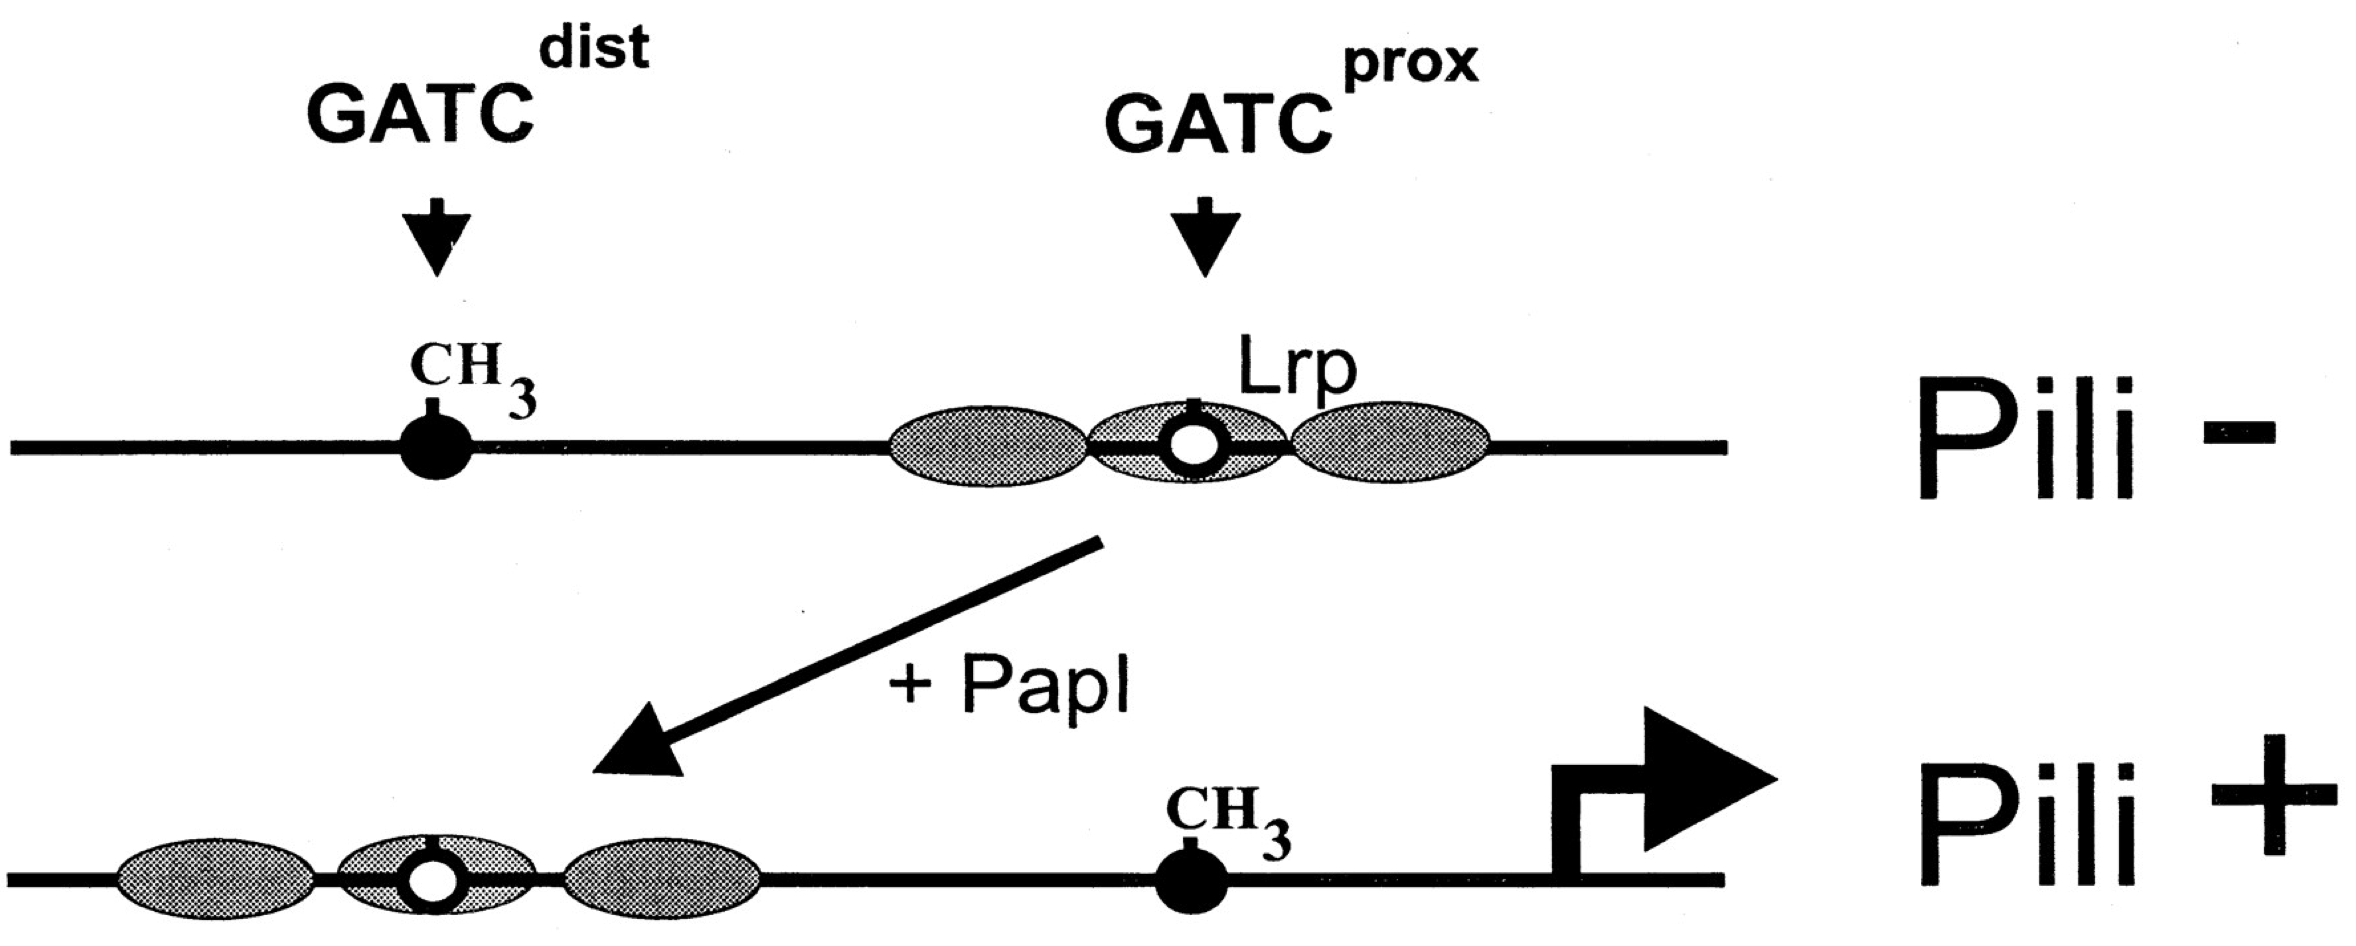
\includegraphics[scale=0.3]{text/Pictures/papPili.png}
    \caption{Scheme of the \tax{pap} phase OFF to ON switch. (reproduced from \cite{low2001roles})}
    \label{pap}
\end{figure}

As implied above several GATC sites escape Dam methylation.
This happens if another regulatory protein recognises a specific DNA binding site which overlaps GATC sequence and thus competes with Dam for it \cite{correnti2002dam}.
Such a mechanism leading to epigenetic switch is well characterized in synthesis of \tax{pap} pili in uropathogenic \tax{E. coli} (UPEC) \cite{peterson2008competitive}.
%%%The regulatory sequence of the \tax{pap} operon contains two sets of Lrp binding sites 1-3 and 4-6.
%%%In both of them the GATC sequence is present, GATC$^{prox}$ within site 2 and GATC$^{dist}$ within site 5 (Fig.~\ref{pap}) \cite{blyn1990regulation}.
The regulatory sequence of the \tax{pap} operon contains two sets of Lrp binding sites GATC$^{prox}$ and GATC$^{dist}$ \cite{blyn1990regulation}.
During the OFF phase \tax{pap} pili are not produced because Lrp occupies GATC$^{prox}$ site which remains nonmethylated on both strands while GATC$^{dist}$ is fully methylated (Fig.~\ref{pap}).
Lrp in this position prevents binding not only by Dam but by $\sigma^{70}$ RNA polymerase as well, inhibiting expression of \tax{papBA} gene \cite{weyand2000regulation}.
For a switch to ON phase an initial Lrp dissociation from GATC$^{prox}$ is necessary.
This likely happens during replication when an opportunity for Lrp to bind the hemimethylated GATC$^{dist}$ site instead of GATC$^{prox}$ raises.
The probability of this switch depends on the level of regulatory protein PapI in the cell as complex PapI/Lrp has lower affinity to GATC$^{prox}$ but binds more likely to hemimethylated GATC$^{dist}$ than to fully methylated DNA \cite{hernday2003mechanism}.
Besides, Lrp release from GATC$^{prox}$ site enables access of Dam to it so it can become methylated which further reduces Lrp affinity to this site.
Even though RNA polymerase's access to \tax{papBA} promoter is not blocked anymore the expression itself requires CRP \cite{weyand2001essential}.
When PapB is being produced it acts as a \tax{papI} gene transcription activator leading to a feedback loop which stabilizes the cells in ON phase \cite{forsman1989autoregulation}.
However, the described transition from OFF to ON phase occurs with 100-fold lower frequency than vice versa \cite{blyn1990regulation}.
The process of this opposite transition, i.e., from ON to OFF phase involves a transfer of Lrp from GATC$^{dist}$ to GATC$^{prox}$ during replication, but the exact mechanism is not fully understood yet \cite{adhikari2016dna}.

%%%Another well known orphan MT in \tax{E. coli} is \textbf{Dcm} which methylates second cytosine in 5'-CC(A/T)GG-3' motif to 5-methylcytosine (5mC) \cite{marinus1973isolation}.
%%%Even though neither this one is necessary for \tax{E. coli} survival and some strains were found lacking \tax{dcm} gene, a link between certain genes expression and presence of this MT was described.
%%%Dcm seems to slow down expression of ribosomal genes \tax{rplC} and \tax{rpsJ} and inhibit transcription of \tax{sugE} gene connected with higher antimicrobial resistance \cite{militello2012conservation, militello2014cytosine}.
%%%Both are happening predominantly during the early stationary phase.
%%%Next study shows increased expression of stress response sigma factor RpoS in \tax{dcm} mutant \cite{kahramanoglou2012genomics}.
%%%Recently additional 63 genes were discovered to be affected if Dcm activity is inhibited \cite{militello20165}.
%%%Most of these genes are up-regulated during early stationary phase if methylation by Dcm is silenced.

%%%Lastly \textbf{YhdJ} is an orphan MT methylating 3' adenine of 5'-ATGCAT-3' sequence to 6mA when overexpressed.
%%%Deleting \tax{yhdJ} gene produces neither loss of viability of \tax{E. coli} nor changes in its phenotype.
%%%In addition, the expression of the gene is very low under usual laboratory conditions, and nothing is known about the transcription regulation of the gene \cite{broadbent2007yhdj}.

%%%\subsubsection{Protein aggregation}
%%%At the end of the previous month a new mechanism of bacterial memory was described.
%%%Protein aggregates (PAs) which are usually formed in response to proteotoxic stress (e.g., sub-lethal heat-shock) were found to protect cells which bear them against new proteotoxic stresses \cite{govers2018protein}.
%%%Those PAs are asymmetrically divided between daughter cells and gradually disaggregated.
%%%As this disaggregation is very slow, it provides a long-time memory in PA-bearing cells of past proteotoxic events.
%%%The authors show that cells which inherit protein aggregates are more likely to survive sub-lethal heat-shock or streptomycin exposure.
%%%They also resume growth much earlier than genetically identical cells without PA.



\section{Predictive cell behaviour}
An ability to predict an upcoming event in the environment can be beneficial.
No matter whether the event means a presence of antibiotic or just a shift in carbon source availability.
If a bacterium is able to predict such an event, it has a fitness advantage over those who do not expect this to happen in that community.
It is so because such cell starts up its expression for the future change in advance which does not cause a delay in response at the time the change emerges.

Circadian rhythms in photoautotrophic Cyanobacteria represent one example of predictive behaviour in bacteria.
It consists of alternation between photosynthetic activity during the day and nitrogen fixation at night.
This periodicity persists in complete darkness or light for days.
It can also be reset by light or dark pulses in a way that two genetically identical populations act in the opposite way (oxygen production or nitrogen fixation) in a constant dark or light conditions at the same time \cite{kondo1993circadian}.
A similar oscillatory rhythm was described in a bacterium other than Cyanobacterium.
\tax{Rhodobacter sphaeroides} also controls gene expression in circadian (aerobic conditions) or ultradian (anaerobic conditions) rhythms \cite{min2005rhythmic}.
A recent study investigating the connection between the day-and-night cycle and overall gene expression of microbial mat suggests that daily rhythmicity might not be uncommon outside Cyanobacteria \cite{hornlein2018daily}.
The authors state that 50\% of the rhythmic genes was derived from phylum \tax{Proteobacteria}.

Predictive behaviour has been observed in \tax{E. coli} as well.
Naturally, it faces recurrent transitions between mammalian gastrointestinal tract (GIT) - higher temperature, lower oxygen - and outside environment - lower temperature, higher oxygen.
\tax{E. coli} strongly represses genes responsible for aerobic metabolism after temperature increase (without a change in oxygen levels) in laboratory conditions \cite{tagkopoulos2008predictive}.
While if the temperature drops, a correlation in up-regulation of aerobic metabolism genes occurs.
They also evolved this strain in conditions where an increase in temperature was followed by oxygen saturation and temperature decrease by anaerobic conditions.
The two responses were successfully decoupled after 1000 generations suggesting that anticipatory regulation can be evolved for and against.

Predictive behaviour in maltose to lactose shift was also described \cite{mitchell2009adaptive}.
Evolution under high lactose concentrations without maltose resulted in the loss in the prediction of maltose exposure and evolved lines exhibit a significant fitness disadvantage compared to ancestor upon lactose-maltose transition.
The same authors investigated anticipation of oxidative stress by yeast which occurs in its natural habitat upon transition from fermentation to respiration.
\tax{Saccharomyces cerevisiae} uses heat-shock, ethanol, and low pH as cues to prepare for its coming environment without actually experiencing it at the time \cite{mitchell2009adaptive}.


\section{Natural selection on responses and memory}
The current knowledge about gene expression in prokaryotes shows that transcription is a fairly regulated process.
However, how this regulation evolved under selection in natural conditions is not yet fully understood yet.

\subsection{Selection on sensitivity}
I mentioned above that cells possess mechanisms to modulate the time-dependent sensitivity of gene expression to a signal (e.g., FFLs).
Some of these mechanisms are overrepresented in living organisms compared to what it would look like in randomized networks \cite{shen2002network, mangan2003structure}.
This suggests that selection has acted to increase the accurate timing of their responses.
But, is concentration-dependent sensitivity to a signal under selective pressure as well?
Generally, there should be selection towards the concentration of a signal that is somehow informative in the particular environment.
However, there has been little work done to address this question so far.
One way to look into whether it is possible for promoter sensitivity to change in response to selection is through experimental evolution.
The sensitivity of promoter variants from natural isolates could be then compared to those of lines evolved under low to high levels of an appropriate signal.
A better way would be a comparison of natural variants to a neutral variation model such as random mutagenesis.
But, looking solely at the distribution of concentration sensitivity of naturally occurring promoters could also provide useful information in this matter.

\subsection{Selection on noise}
In the case of expression noise, prior works have clearly shown that it is an evolvable trait \cite{richard2014does}.
Generally, essential, constitutional genes and genes with high effect on overall expression (i.e., some transcription factors) tend to have low transcriptional noise \cite{silander2012genome, metzger2015selection}.
In contrast, another interesting study describes higher noise in promoters from natural isolates of \tax{E. coli} compared to those of experimentally evolved lines just for their mean expression \cite{wolf2015expression}.
These results suggest that for different genes and/or at different niches there is a different optimum of transcriptional noise.
Indeed, a very recent study of the effect of expression noise on the fitness of \tax{Saccharomyces cerevisiae} reveals that high noise is beneficial when the expression level is far from optimum and vice versa \cite{duveau2018fitness}.
They also indicate that after the introduction of an organism into a new environment selection might act towards high noise in the expression of some genes before appropriate expression plasticity evolves.
However, note that mutations in promoter regions usually change both expression level and noise at the same time \cite{metzger2015selection}.
Some work in this area on other model organisms such as \tax{Drosophila melanogaster} \cite{schor2017promoter} and mouse \cite{barroso2017evolution} has been done as well.
But, it remains to validate that it is actually selected for certain levels of noise in the natural environment.
This could be done by looking into noise variations of individual genes among distinct microbial isolates coming from the same location.

\subsection{Selection on memory}
It is known that some bacteria can react faster to a signal if they were exposed to the same signal in past \cite{novick1957enzyme}.
For example, sister and cousin cells have correlated lag times upon glucose-lactose media switch \cite{boulineau2013single, kaiser2018monitoring}.
LacY production in \tax{E. coli} continues after a short lactose pulse although the lactose is no longer present \cite{lambert2014memory} and \tax{E. coli} also keeps producing more LacZ even after reaching maximal growth rate and thus overshooting its actual need \cite{kaiser2018monitoring}.
Similar behaviour was observed in yeast galactose system \cite{zacharioudakis2007yeast, razinkov2013measuring}.
But, a question remains: are these observed traits indeed what is actively selected for in a natural fluctuating environment in order to remember past events for several generations?

Some bacteria are also able to predict upcoming event based on otherwise unrelated signal \cite{kondo1993circadian, min2005rhythmic, tagkopoulos2008predictive, mitchell2009adaptive}.
An attempt of an evolution of classical Pavlovian reflex to initially neutral signal in microorganisms was published last year \cite{lopez2017adaptive}.
Caffeine was added to the media as the neutral signal and yeast \tax{S. cerevisiae} was expected to associate it with the upcoming 5-fluoroorotic acid presence (metabolised into a toxic substance).
This predictive-like response appeared just within a few hundred generations but was not stable over time.
Thus, little is still known how microorganisms evolve such reflex to neutral cues.
A mathematical model suggests this to occur if benefits of such prediction exceed its costs in other environments \cite{mitchell2011mathematical}, but no experimental evidence is available so far.
Nevertheless, the decoupling of reaction to a signal in the absence of expected outcome reported previously is an indication of selection acting on predictive behaviour \cite{tagkopoulos2008predictive, mitchell2009adaptive}.

Almost all work on bacterial responses, memory and predictive behaviour has been performed on lab strains and by using just a single strain of a particular genus.
However, the questions about how natural selection acts on transcriptional responses and memory in bacteria cannot be fully addressed without exploring natural variability in individual promoters among various isolates of the same genus.
Because without the knowledge of the natural phenotypic and genotypic variation in responses and memory we can only guess how selection forces shape these traits in nature, at what extent or whether they really do so.
And this is something no one has looked into in detail as yet.

Here I will investigate how selection acts on these traits by quantifying them in natural isolates of \tax{E. coli} and comparing these to a neutral model of variation generated in the lab.
By testing whether the observed variants have lower or higher levels of divergence than randomly selected variants we can infer how natural selection is acting.
I detail these approaches in the following section.

%%%\section{Natural variation in responses and memory}
%%%Although the presence of \tax{E. coli} in water is still widely used as an indicator of fecal contamination, recent studies show that some \tax{E. coli} isolates are able to reproduce in outside environment \cite{byappanahalli2004indigenous, somorin2016general}.
%%%Moreover, strains inhabiting soil for a long time were found to be distinctive from those isolated from animals \cite{walk2009cryptic, walk2015cryptic}.
%%%This raises the questions how these bacteria survive outside their hosts.
%%%The ability of \tax{E. coli} to adapt to such different environments as animal gut and soil or water are, might also help us understand the evolution of promoters to fluctuating environments and bacterial memory.
%%%
%%%When looking at the adaptation of a species to various conditions, one should consider not only genotypic but phenotypic variation as well.
%%%It is now well known and generally accepted that even cells with the same genotype do not necessarily exhibit the same phenotype in identical conditions \cite{ronin2017long, govers2018protein}.
%%%On the other hand, various genetic backgrounds might still have a very similar phenotype in some cases if evolution in the environment with strong selection occurs.
%%%In other words, various strains might come to the same phenotype by different genotypic solutions.

\cleardoublepage%%% keeps correct headings

\shorthandon{-}
%%%%%%%%%%%%%%%%%%%%%%%%%%%%%%%%%%%%
